In this chapter, the object allocation framework from \autoref{sec:alloc} is applied to four OCELs available in the OCEL~2.0 format.
The evaluation of the allocation rules addresses \RGfourB{} by analyzing their allocation results and runtime performance. Furthermore, it assesses influences of event log characteristics on these outcomes.
%
After explaining the evaluation setup (\autoref{sec:eva-setup}), the input data are summarized (\autoref{sec:eva-input}). The results are given in \autoref{sec:eva-results}.

% ---------------------------------------------------------------------
% ---------------------------------------------------------------------
\section{Setup}
\label{sec:eva-setup}
% ---------------------------------------------------------------------
% ---------------------------------------------------------------------

The evaluation consists of two parts.
The first part examines characteristics of the resulting emission distributions. In the second part, the runtime of the \allocrule{ClosestTargets} rule is analyzed.
The experiments are conducted on four OCELs which are introduced after defining the setup.
%
The assignments of the datasets' object types to HU or resource are given and justified in the dedicated result sections.
Each object type is tested as target object type, with the exception of those types that only have one object, as allocation results are trivial in this case. For an object type $\ot\in\OTL$ with at least two objects, this leads to
$\Omega\coloneqq \{ o\in O \mid \objtype(o)=\ot \}$.
The experiment is repeated for each of these target object type settings.

On these input data, different allocation rules are applied:
\allocrule{AllTargets} ($\alphaAT$),
\allocrule{ParticipatingTargets} ($\alphaPT$)
and \allocrule{ClosestTargets} ($\alphaCTall$).
%
The \allocrule{ClosestTargets} rule is applied repeatedly, testing all four object interaction graphs defined in \autoref{sec:alloc-og}.
Depending on the graph, the rule is abbreviated as follows:
\begin{itemize}
  \item CT: Full object interaction graph ($\OGOmegaL$),
  \item CTx: Full object interaction graph without object type self-loops ($\OGxOmegaL$),
  \item CTHU: HU interaction graph ($\OGHUOmegaL$),
  \item CTHUx: HU interaction graph without object type self-loops ($\OGHUxOmegaL$).
\end{itemize}

The graphs without object type self-loops are created in order to reduce the edge count and thus speed up distance computation.
We claim that the allocation results are the same regardless of using an object interaction graph with or without object type self-loops. This claim is to be verified in the experiment for the given OCELs and sets of target object types.

\begin{figure}[t]
  \begin{small}
    \begin{center}
      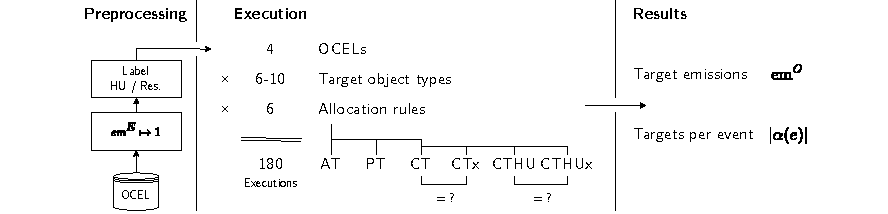
\includegraphics[width=0.95\textwidth]{figures/concept/evaluation.drawio.pdf}
    \end{center}
    \caption{Schematic overview of the evaluation procedure. In total, 180 different combinations of input data and parameters are tested. Next to the \allocrule{AllTargets} and \allocrule{ParticipatingTargets} rules, \allocrule{ClosestTargets} is tested with the four different object interaction graphs. The target emissions $\emO$ and number of targets per event $|\alpha(e)|$ are saved as results for further analysis.}
    \label{fig:eva-setup}
  \end{small}
\end{figure}

\autoref{fig:eva-setup} shows an overview of this procedure, highlighting the number of different input datasets and execution parameters.
The experiment is repeated for every OCEL and for every object type as target object type.
The result of each execution is the target object emission distribution and the number of targets per event, additionally containing the distance at which they are found in the selected object interaction graph when using the \allocrule{ClosestTargets} rule.

% ---------------------------------------------------------------------
\subsection{Target Emission Distribution}
\label{ssec:eva-setup-distr}
% ---------------------------------------------------------------------

The goal of this experiment is to evaluate the allocation rules and the resulting target object emissions and to relate these results to characteristics of the input data.
Because of this, the event emissions are set to \qty{1}{\kgcotwoe} per event, with no E2O emissions, leading to $\emRem(e) = 1 \;\forall e \in E$. This prevents potential influence of event emission variance on the resulting object emissions.

The allocation results are further processed, computing measures used for comparison.
The list of measures is shown in \autoref{tab:eva-setup-stats}.
The variation coefficient ($\cv$) measures the relative variance of target emissions.
It is chosen over standard deviation because the emissions per target deviate by magnitudes depending on both the overall emissions (due to different numbers of events),
and the number of target objects. Thus, comparability between results for different target object types is guaranteed.
%
The number of target objects an event is allocated to indicates among how many objects the emissions are distributed.
Two extreme cases are events that get allocated uniquely (to one target) or uniformly (to all targets), as introduced in \autoref{sec:alloc-props}.
These measures are included as well as the median number of targets per event ($\abs{\alpha(e)}_{50}$).
%
For the \allocrule{ClosestTargets} rule, additional measures based on the selected object interaction graph $\OG$ are computed.
The distances of shortest paths to target objects used for allocation provide information on how target objects are located in the graph. The maximum of these distances ($d^E_{\max}$) is included.
Degrees in the object interaction graph differ between the full and HU interaction graph as resources have higher degrees than HUs. This difference is assessed by giving the median and maximum degrees of all objects ($\deg_{50}, \deg_{\max}$) and target objects only ($\deg^\Omega_{50}, \deg^\Omega_{\max}$).
% with the latter jointly providing statistics per object type as all are selected as target objects in different runs.
Lastly, the number of edges ($\abs{\Edges(\OG)}$) and connected components ($\abs{\Comp(\OG)}$) are given to compare size and connectivity of the different graphs.

\begin{table}[t]
  \begin{small}
    \caption{Statistics computed for all allocation results. For allocation with the \allocrule{ClosestTargets} rule, additional statistics based on the object interaction graph $\OG$ are computed.}
    \label{tab:eva-setup-stats}
    \begin{center}
      \begin{tabularx}{\textwidth}{llX}
        \toprule
        \textbf{Statistic} & \textbf{Symbol} & \textbf{Rules} \\
        \midrule
        Variation coefficient of target object emissions
        & $\cv$ & all \\
        Number of target objects per event (median)
        & $\abs{\alpha(e)}_{50}$ & all \\
        Fraction of events uniformly allocated
        & $\funiformalpha$ & all \\
        Fraction of events uniquely allocated
        & $\funiquealpha$ & all \\
        Distances of shortest paths used for event allocation (max.)
        & $\dist{\max}^E$ & CT\dots \\
        Degrees in object interaction graph (med. / max.)
        & $\deg_{50}, \deg_{\max}$ & CT\dots \\
        Degrees of targets in object interaction graph (med. / max.)
        & $\deg^\Omega_{50}, \deg^\Omega_{\max}$ & CT\dots \\
        Number of edges / components in object interaction graph
        & $\abs{\Edges(\OG)}, \abs{\Comp(\OG)}$ & CT\dots \\
        \bottomrule
      \end{tabularx}
    \end{center}
  \end{small}
\end{table}

% ---------------------------------------------------------------------
\subsection{Runtime Analysis}
\label{ssec:eva-setup-runtime}
% ---------------------------------------------------------------------

The \allocrule{ClosestTargets} allocation rule involves computing distances on an object interaction graph.
As opposed to the other allocation rules, the computation time is potentially high for large datasets.
In the following, a runtime experiment is conducted, repeatedly executing allocation rules on all input data and configurations from the first experiment.
Each configuration is tested three times, capturing the minimum runtime.

As the graph is unweighted and only shortest distances to any target object are requested,
distances are computed by means of breadth-first search (BFS).
For processing and saving the underlying graph structure, the \texttt{networkx} Python library is utilized.
A custom BFS algorithm is implemented that allows for early stopping once a target object has been found, except for processing all objects at the same distance.
Distances are first computed between pairs of objects.
After that, closest targets are looked up for the objects participating in each event, resulting in a set of closest targets per event.

The experiments are conducted on a system running Ubuntu 24.04 with an Intel i7-14700K processor (16 cores: 8x \qty{5.3}{\giga\hertz}, 8x \qty{4.2}{\giga\hertz}) and \qty{32}{\giga\byte} DDR5-\qty{6000}{\mega\hertz} CL36 RAM.

% ---------------------------------------------------------------------
% ---------------------------------------------------------------------
\section{Input Data}
\label{sec:eva-input}
% ---------------------------------------------------------------------
% ---------------------------------------------------------------------

To evaluate the allocation technique, different OCELs are used as input data.
Given that OCPM is a novel concept, the availability of real-world datasets is limited.
Alongside the OCEL~2.0 standard~\cite{OCEL2}, three simulated event logs have been published, based on order management~\cite{orderManagement}, container logistics~\cite{containerLogistics}, and Purchase-to-Pay (P2P)~\cite{p2p} processes.
Each of these OCELs contains about 10k objects and between 14k and 36k events.
The only real-world dataset published with the OCEL~2.0 standard is not considered, as it refers to the history of a git repository which is not considered relevant for emission analysis~\cite{angularCommits}.

Another OCEL used for evaluation has been developed to exemplify the integration of sustainability data, including carbon equivalents of events and objects, into OCELs.
This dataset is based on a hinge manufacturing process and is the largest dataset used for evaluation, containing 24k objects and 39k events~\cite{hinge}.

Details about the underlying processes and object relations of the individual OCEls are given in dedicated sections of~\autoref{sec:eva-results}, followed by results specific to that dataset.

% ---------------------------------------------------------------------
% ---------------------------------------------------------------------
\begin{landscape}
  \midsepsymmetric
  
% Feedback:
% - highlight HU/Res target types
%     idea: <ot> (HU) (right/left aligned columns)
% - vertical lines
% - top titles centered

\begin{table}[t]
  \centering
  \caption{Results of the allocation evaluation. For each target object type setting ($\mathit{OT}_\Omega$), the rules \allocrule{AllTargets}, \allocrule{ParticipatingTargets}, and \allocrule{ClosestTargets} with full (CT) and HU graph (CTHU) are applied. The table includes the variation coefficient of target emissions ($\cv$), the median number of targets per event ($|\alpha(e)|_{50}$), the percentages of events allocated uniquely ($\funiquealpha$) and uniformly ($\funiformalpha$), and the maximal graph distance used to allocate events ($\dist{\max}^E$).}
  \label{tab:eva-results-alloc}
  \footnotesize
  \begin{tabular}{lr@{\ }lrrrrrllllrrrrrrrrrr}
    \toprule
    &&& $|\Omega|$ & \multicolumn{4}{c}{$\cv$} & \multicolumn{4}{c}{$|\alpha(e)|_{50}$} & \multicolumn{4}{c}{$\funiquealpha$ [\%]} & \multicolumn{4}{c}{$\funiformalpha$ [\%]} & \multicolumn{2}{c}{$\dist{\max}^E$} \\
    $L$ & $\OT_\Omega$ &&& \scriptsize AT & \scriptsize PT & \scriptsize CT & \scriptsize\hspace*{-.5em}CTHU\hspace*{-.5em} & \scriptsize AT & \scriptsize PT & \scriptsize CT & \scriptsize\hspace*{-.5em}CTHU\hspace*{-.5em} & \scriptsize AT & \scriptsize PT & \scriptsize CT & \scriptsize\hspace*{-.5em}CTHU\hspace*{-.5em} & \scriptsize AT & \scriptsize PT & \scriptsize CT & \scriptsize\hspace*{-.5em}CTHU\hspace*{-.5em} & \scriptsize CT & \scriptsize\hspace*{-.5em}CTHU\hspace*{-.5em} \\
    \midrule
    \multirow[c]{6}{*}{\makecell[l]{Ord.\\Mgmt.}} & item & {\scriptsize (HU)} & 7659 & {\cellcolor[HTML]{0B0000}} \color[HTML]{F1F1F1} .00 & {\cellcolor[HTML]{FF4F00}} \color[HTML]{F1F1F1} .39 & {\cellcolor[HTML]{FF4F00}} \color[HTML]{F1F1F1} .39 & {\cellcolor[HTML]{FF4F00}} \color[HTML]{F1F1F1} .39 & {\cellcolor[HTML]{A50026}} \color[HTML]{F1F1F1} all & {\cellcolor[HTML]{006837}} \color[HTML]{F1F1F1} 1 & {\cellcolor[HTML]{006837}} \color[HTML]{F1F1F1} 1 & {\cellcolor[HTML]{006837}} \color[HTML]{F1F1F1} 1 & {\cellcolor[HTML]{F7FCF5}} \color[HTML]{000000} \num{0} & {\cellcolor[HTML]{63BC6E}} \color[HTML]{F1F1F1} \num{54} & {\cellcolor[HTML]{63BC6E}} \color[HTML]{F1F1F1} \num{54} & {\cellcolor[HTML]{63BC6E}} \color[HTML]{F1F1F1} \num{54} & {\cellcolor[HTML]{67000D}} \color[HTML]{F1F1F1} \num{100} & {\cellcolor[HTML]{FFF5F0}} \color[HTML]{000000} \num{0} & {\cellcolor[HTML]{FFF5F0}} \color[HTML]{000000} \num{0} & {\cellcolor[HTML]{FFF5F0}} \color[HTML]{000000} \num{0} & {\cellcolor[HTML]{440154}} \color[HTML]{F1F1F1} 0 & {\cellcolor[HTML]{440154}} \color[HTML]{F1F1F1} 0 \\
    & ord & {\scriptsize (HU)} & 2000 & {\cellcolor[HTML]{0B0000}} \color[HTML]{F1F1F1} .00 & {\cellcolor[HTML]{3A0000}} \color[HTML]{F1F1F1} .06 & {\cellcolor[HTML]{FF0500}} \color[HTML]{F1F1F1} .30 & {\cellcolor[HTML]{FF4C00}} \color[HTML]{F1F1F1} .38 & {\cellcolor[HTML]{A50026}} \color[HTML]{F1F1F1} all & {\cellcolor[HTML]{A50026}} \color[HTML]{F1F1F1} all & {\cellcolor[HTML]{F7814C}} \color[HTML]{F1F1F1} 345 & {\cellcolor[HTML]{006837}} \color[HTML]{F1F1F1} 1 & {\cellcolor[HTML]{F7FCF5}} \color[HTML]{000000} \num{0} & {\cellcolor[HTML]{B4E1AD}} \color[HTML]{000000} \num{31} & {\cellcolor[HTML]{B4E1AD}} \color[HTML]{000000} \num{31} & {\cellcolor[HTML]{0B7734}} \color[HTML]{F1F1F1} \num{84} & {\cellcolor[HTML]{67000D}} \color[HTML]{F1F1F1} \num{100} & {\cellcolor[HTML]{DD2A25}} \color[HTML]{F1F1F1} \num{69} & {\cellcolor[HTML]{FFF5F0}} \color[HTML]{000000} \num{0} & {\cellcolor[HTML]{FFF5F0}} \color[HTML]{000000} \num{0} & {\cellcolor[HTML]{472D7B}} \color[HTML]{F1F1F1} 1 & {\cellcolor[HTML]{472D7B}} \color[HTML]{F1F1F1} 1 \\
    & pckg & {\scriptsize (HU)} & 1128 & {\cellcolor[HTML]{0B0000}} \color[HTML]{F1F1F1} .00 & {\cellcolor[HTML]{270000}} \color[HTML]{F1F1F1} .04 & {\cellcolor[HTML]{B00000}} \color[HTML]{F1F1F1} .20 & {\cellcolor[HTML]{FF3F00}} \color[HTML]{F1F1F1} .37 & {\cellcolor[HTML]{A50026}} \color[HTML]{F1F1F1} all & {\cellcolor[HTML]{A50026}} \color[HTML]{F1F1F1} all & {\cellcolor[HTML]{D93429}} \color[HTML]{F1F1F1} 526 & {\cellcolor[HTML]{006837}} \color[HTML]{F1F1F1} 1 & {\cellcolor[HTML]{F7FCF5}} \color[HTML]{000000} \num{0} & {\cellcolor[HTML]{D9F0D3}} \color[HTML]{000000} \num{18} & {\cellcolor[HTML]{D9F0D3}} \color[HTML]{000000} \num{18} & {\cellcolor[HTML]{1E8741}} \color[HTML]{F1F1F1} \num{77} & {\cellcolor[HTML]{67000D}} \color[HTML]{F1F1F1} \num{100} & {\cellcolor[HTML]{B51318}} \color[HTML]{F1F1F1} \num{82} & {\cellcolor[HTML]{FFF5F0}} \color[HTML]{000000} \num{0} & {\cellcolor[HTML]{FFF5F0}} \color[HTML]{000000} \num{0} & {\cellcolor[HTML]{472D7B}} \color[HTML]{F1F1F1} 1 & {\cellcolor[HTML]{472D7B}} \color[HTML]{F1F1F1} 1 \\
    & cust & {\scriptsize (Res.)} & 15 & {\cellcolor[HTML]{0B0000}} \color[HTML]{F1F1F1} .00 & {\cellcolor[HTML]{1A0000}} \color[HTML]{F1F1F1} .02 & {\cellcolor[HTML]{1A0000}} \color[HTML]{F1F1F1} .02 & {\cellcolor[HTML]{590000}} \color[HTML]{F1F1F1} .09 & {\cellcolor[HTML]{A50026}} \color[HTML]{F1F1F1} all & {\cellcolor[HTML]{A50026}} \color[HTML]{F1F1F1} all & {\cellcolor[HTML]{A50026}} \color[HTML]{F1F1F1} all & {\cellcolor[HTML]{006837}} \color[HTML]{F1F1F1} 1 & {\cellcolor[HTML]{F7FCF5}} \color[HTML]{000000} \num{0} & {\cellcolor[HTML]{D6EFD0}} \color[HTML]{000000} \num{19} & {\cellcolor[HTML]{D6EFD0}} \color[HTML]{000000} \num{19} & {\cellcolor[HTML]{00441B}} \color[HTML]{F1F1F1} \num{100} & {\cellcolor[HTML]{67000D}} \color[HTML]{F1F1F1} \num{100} & {\cellcolor[HTML]{B81419}} \color[HTML]{F1F1F1} \num{81} & {\cellcolor[HTML]{B81419}} \color[HTML]{F1F1F1} \num{81} & {\cellcolor[HTML]{FFF5F0}} \color[HTML]{000000} \num{0} & {\cellcolor[HTML]{472D7B}} \color[HTML]{F1F1F1} 1 & {\cellcolor[HTML]{472D7B}} \color[HTML]{F1F1F1} 1 \\
    & empl & {\scriptsize (Res.)} & 18 & {\cellcolor[HTML]{0B0000}} \color[HTML]{F1F1F1} .00 & {\cellcolor[HTML]{FFFF0B}} \color[HTML]{000000} .60 & {\cellcolor[HTML]{FFFF0B}} \color[HTML]{000000} .60 & {\cellcolor[HTML]{FFFF91}} \color[HTML]{000000} .71 & {\cellcolor[HTML]{A50026}} \color[HTML]{F1F1F1} all & {\cellcolor[HTML]{006837}} \color[HTML]{F1F1F1} 1 & {\cellcolor[HTML]{006837}} \color[HTML]{F1F1F1} 1 & {\cellcolor[HTML]{006837}} \color[HTML]{F1F1F1} 1 & {\cellcolor[HTML]{F7FCF5}} \color[HTML]{000000} \num{0} & {\cellcolor[HTML]{278F48}} \color[HTML]{F1F1F1} \num{73} & {\cellcolor[HTML]{278F48}} \color[HTML]{F1F1F1} \num{73} & {\cellcolor[HTML]{278F48}} \color[HTML]{F1F1F1} \num{73} & {\cellcolor[HTML]{67000D}} \color[HTML]{F1F1F1} \num{100} & {\cellcolor[HTML]{FDC5AE}} \color[HTML]{000000} \num{22} & {\cellcolor[HTML]{FDC5AE}} \color[HTML]{000000} \num{22} & {\cellcolor[HTML]{FFF5F0}} \color[HTML]{000000} \num{0} & {\cellcolor[HTML]{472D7B}} \color[HTML]{F1F1F1} 1 & {\cellcolor[HTML]{472D7B}} \color[HTML]{F1F1F1} 1 \\
    & prod & {\scriptsize (Res.)} & 20 & {\cellcolor[HTML]{0B0000}} \color[HTML]{F1F1F1} .00 & {\cellcolor[HTML]{3A0000}} \color[HTML]{F1F1F1} .06 & {\cellcolor[HTML]{3A0000}} \color[HTML]{F1F1F1} .06 & {\cellcolor[HTML]{3A0000}} \color[HTML]{F1F1F1} .06 & {\cellcolor[HTML]{A50026}} \color[HTML]{F1F1F1} all & {\cellcolor[HTML]{006837}} \color[HTML]{F1F1F1} 1 & {\cellcolor[HTML]{006837}} \color[HTML]{F1F1F1} 1 & {\cellcolor[HTML]{006837}} \color[HTML]{F1F1F1} 1 & {\cellcolor[HTML]{F7FCF5}} \color[HTML]{000000} \num{0} & {\cellcolor[HTML]{62BB6D}} \color[HTML]{F1F1F1} \num{54} & {\cellcolor[HTML]{62BB6D}} \color[HTML]{F1F1F1} \num{54} & {\cellcolor[HTML]{62BB6D}} \color[HTML]{F1F1F1} \num{54} & {\cellcolor[HTML]{67000D}} \color[HTML]{F1F1F1} \num{100} & {\cellcolor[HTML]{FFF5F0}} \color[HTML]{000000} \num{0} & {\cellcolor[HTML]{FFF5F0}} \color[HTML]{000000} \num{0} & {\cellcolor[HTML]{FFF5F0}} \color[HTML]{000000} \num{0} & {\cellcolor[HTML]{440154}} \color[HTML]{F1F1F1} 0 & {\cellcolor[HTML]{440154}} \color[HTML]{F1F1F1} 0 \\%
    \midrule%
    \multirow[c]{7}{*}{\makecell[l]{Ctr.\\Log.}} & Ctr & {\scriptsize (HU)} & 1996 & {\cellcolor[HTML]{0B0000}} \color[HTML]{F1F1F1} .00 & {\cellcolor[HTML]{510000}} \color[HTML]{F1F1F1} .09 & {\cellcolor[HTML]{960000}} \color[HTML]{F1F1F1} .17 & {\cellcolor[HTML]{960000}} \color[HTML]{F1F1F1} .17 & {\cellcolor[HTML]{A50026}} \color[HTML]{F1F1F1} all & {\cellcolor[HTML]{006837}} \color[HTML]{F1F1F1} 1 & {\cellcolor[HTML]{006837}} \color[HTML]{F1F1F1} 1 & {\cellcolor[HTML]{006837}} \color[HTML]{F1F1F1} 1 & {\cellcolor[HTML]{F7FCF5}} \color[HTML]{000000} \num{0} & {\cellcolor[HTML]{3FA95C}} \color[HTML]{F1F1F1} \num{63} & {\cellcolor[HTML]{005A24}} \color[HTML]{F1F1F1} \num{93} & {\cellcolor[HTML]{005A24}} \color[HTML]{F1F1F1} \num{93} & {\cellcolor[HTML]{67000D}} \color[HTML]{F1F1F1} \num{100} & {\cellcolor[HTML]{FC9B7C}} \color[HTML]{000000} \num{35} & {\cellcolor[HTML]{FFF5F0}} \color[HTML]{000000} \num{0} & {\cellcolor[HTML]{FFF5F0}} \color[HTML]{000000} \num{0} & {\cellcolor[HTML]{3B528B}} \color[HTML]{F1F1F1} 2 & {\cellcolor[HTML]{3B528B}} \color[HTML]{F1F1F1} 2 \\
    & CO & {\scriptsize (HU)} & 600 & {\cellcolor[HTML]{0B0000}} \color[HTML]{F1F1F1} .00 & {\cellcolor[HTML]{0B0000}} \color[HTML]{F1F1F1} .00 & {\cellcolor[HTML]{FF4C00}} \color[HTML]{F1F1F1} .38 & {\cellcolor[HTML]{FF4C00}} \color[HTML]{F1F1F1} .38 & {\cellcolor[HTML]{A50026}} \color[HTML]{F1F1F1} all & {\cellcolor[HTML]{A50026}} \color[HTML]{F1F1F1} all & {\cellcolor[HTML]{006837}} \color[HTML]{F1F1F1} 6 & {\cellcolor[HTML]{006837}} \color[HTML]{F1F1F1} 6 & {\cellcolor[HTML]{F7FCF5}} \color[HTML]{000000} \num{0} & {\cellcolor[HTML]{F2FAF0}} \color[HTML]{000000} \num{3} & {\cellcolor[HTML]{EBF7E7}} \color[HTML]{000000} \num{9} & {\cellcolor[HTML]{EBF7E7}} \color[HTML]{000000} \num{9} & {\cellcolor[HTML]{67000D}} \color[HTML]{F1F1F1} \num{100} & {\cellcolor[HTML]{77040F}} \color[HTML]{F1F1F1} \num{97} & {\cellcolor[HTML]{FFF5F0}} \color[HTML]{000000} \num{0} & {\cellcolor[HTML]{FFF5F0}} \color[HTML]{000000} \num{0} & {\cellcolor[HTML]{2C728E}} \color[HTML]{F1F1F1} 3 & {\cellcolor[HTML]{2C728E}} \color[HTML]{F1F1F1} 3 \\
    & HU & {\scriptsize (HU)} & 10552 & {\cellcolor[HTML]{0B0000}} \color[HTML]{F1F1F1} .00 & {\cellcolor[HTML]{0B0000}} \color[HTML]{F1F1F1} .00 & {\cellcolor[HTML]{810000}} \color[HTML]{F1F1F1} .14 & {\cellcolor[HTML]{980000}} \color[HTML]{F1F1F1} .17 & {\cellcolor[HTML]{A50026}} \color[HTML]{F1F1F1} all & {\cellcolor[HTML]{006837}} \color[HTML]{F1F1F1} 1 & {\cellcolor[HTML]{006837}} \color[HTML]{F1F1F1} 1 & {\cellcolor[HTML]{006837}} \color[HTML]{F1F1F1} 1 & {\cellcolor[HTML]{F7FCF5}} \color[HTML]{000000} \num{0} & {\cellcolor[HTML]{4DB163}} \color[HTML]{F1F1F1} \num{60} & {\cellcolor[HTML]{46AE60}} \color[HTML]{F1F1F1} \num{61} & {\cellcolor[HTML]{45AD5F}} \color[HTML]{F1F1F1} \num{61} & {\cellcolor[HTML]{67000D}} \color[HTML]{F1F1F1} \num{100} & {\cellcolor[HTML]{FC8969}} \color[HTML]{F1F1F1} \num{40} & {\cellcolor[HTML]{FFF5F0}} \color[HTML]{000000} \num{0} & {\cellcolor[HTML]{FFF5F0}} \color[HTML]{000000} \num{0} & {\cellcolor[HTML]{21918C}} \color[HTML]{F1F1F1} 4 & {\cellcolor[HTML]{2C728E}} \color[HTML]{F1F1F1} 3 \\
    & TD & {\scriptsize (HU)} & 594 & {\cellcolor[HTML]{0B0000}} \color[HTML]{F1F1F1} .00 & {\cellcolor[HTML]{0D0000}} \color[HTML]{F1F1F1} .01 & {\cellcolor[HTML]{FF3F00}} \color[HTML]{F1F1F1} .37 & {\cellcolor[HTML]{FF3F00}} \color[HTML]{F1F1F1} .37 & {\cellcolor[HTML]{A50026}} \color[HTML]{F1F1F1} all & {\cellcolor[HTML]{A50026}} \color[HTML]{F1F1F1} all & {\cellcolor[HTML]{006837}} \color[HTML]{F1F1F1} 6 & {\cellcolor[HTML]{006837}} \color[HTML]{F1F1F1} 6 & {\cellcolor[HTML]{F7FCF5}} \color[HTML]{000000} \num{0} & {\cellcolor[HTML]{F0F9EC}} \color[HTML]{000000} \num{5} & {\cellcolor[HTML]{EBF7E7}} \color[HTML]{000000} \num{9} & {\cellcolor[HTML]{EBF7E7}} \color[HTML]{000000} \num{9} & {\cellcolor[HTML]{67000D}} \color[HTML]{F1F1F1} \num{100} & {\cellcolor[HTML]{820711}} \color[HTML]{F1F1F1} \num{95} & {\cellcolor[HTML]{FFF5F0}} \color[HTML]{000000} \num{0} & {\cellcolor[HTML]{FFF5F0}} \color[HTML]{000000} \num{0} & {\cellcolor[HTML]{3B528B}} \color[HTML]{F1F1F1} 2 & {\cellcolor[HTML]{3B528B}} \color[HTML]{F1F1F1} 2 \\
    & Vcl & {\scriptsize (HU)} & 127 & {\cellcolor[HTML]{0B0000}} \color[HTML]{F1F1F1} .00 & {\cellcolor[HTML]{250000}} \color[HTML]{F1F1F1} .03 & {\cellcolor[HTML]{FF5600}} \color[HTML]{F1F1F1} .39 & {\cellcolor[HTML]{FF9000}} \color[HTML]{000000} .46 & {\cellcolor[HTML]{A50026}} \color[HTML]{F1F1F1} all & {\cellcolor[HTML]{A50026}} \color[HTML]{F1F1F1} all & {\cellcolor[HTML]{006837}} \color[HTML]{F1F1F1} 1 & {\cellcolor[HTML]{006837}} \color[HTML]{F1F1F1} 1 & {\cellcolor[HTML]{F7FCF5}} \color[HTML]{000000} \num{0} & {\cellcolor[HTML]{EDF8E9}} \color[HTML]{000000} \num{7} & {\cellcolor[HTML]{147E3A}} \color[HTML]{F1F1F1} \num{80} & {\cellcolor[HTML]{005020}} \color[HTML]{F1F1F1} \num{96} & {\cellcolor[HTML]{67000D}} \color[HTML]{F1F1F1} \num{100} & {\cellcolor[HTML]{8C0912}} \color[HTML]{F1F1F1} \num{92} & {\cellcolor[HTML]{FEEAE1}} \color[HTML]{000000} \num{6} & {\cellcolor[HTML]{FFF2EC}} \color[HTML]{000000} \num{2} & {\cellcolor[HTML]{28AE80}} \color[HTML]{F1F1F1} 5 & {\cellcolor[HTML]{2C728E}} \color[HTML]{F1F1F1} 3 \\
    & FL & {\scriptsize (Res.)} & 3 & {\cellcolor[HTML]{0B0000}} \color[HTML]{F1F1F1} .00 & {\cellcolor[HTML]{0B0000}} \color[HTML]{F1F1F1} .00 & {\cellcolor[HTML]{150000}} \color[HTML]{F1F1F1} .01 & {\cellcolor[HTML]{150000}} \color[HTML]{F1F1F1} .01 & {\cellcolor[HTML]{A50026}} \color[HTML]{F1F1F1} all & {\cellcolor[HTML]{A50026}} \color[HTML]{F1F1F1} all & {\cellcolor[HTML]{006837}} \color[HTML]{F1F1F1} 2 & {\cellcolor[HTML]{006837}} \color[HTML]{F1F1F1} 2 & {\cellcolor[HTML]{F7FCF5}} \color[HTML]{000000} \num{0} & {\cellcolor[HTML]{CFECC9}} \color[HTML]{000000} \num{22} & {\cellcolor[HTML]{75C477}} \color[HTML]{000000} \num{50} & {\cellcolor[HTML]{75C477}} \color[HTML]{000000} \num{50} & {\cellcolor[HTML]{67000D}} \color[HTML]{F1F1F1} \num{100} & {\cellcolor[HTML]{C1161B}} \color[HTML]{F1F1F1} \num{78} & {\cellcolor[HTML]{FEEAE0}} \color[HTML]{000000} \num{7} & {\cellcolor[HTML]{FEEAE1}} \color[HTML]{000000} \num{7} & {\cellcolor[HTML]{28AE80}} \color[HTML]{F1F1F1} 5 & {\cellcolor[HTML]{21918C}} \color[HTML]{F1F1F1} 4 \\
    & Trk & {\scriptsize (Res.)} & 6 & {\cellcolor[HTML]{0B0000}} \color[HTML]{F1F1F1} .00 & {\cellcolor[HTML]{0D0000}} \color[HTML]{F1F1F1} .01 & {\cellcolor[HTML]{150000}} \color[HTML]{F1F1F1} .01 & {\cellcolor[HTML]{150000}} \color[HTML]{F1F1F1} .01 & {\cellcolor[HTML]{A50026}} \color[HTML]{F1F1F1} all & {\cellcolor[HTML]{A50026}} \color[HTML]{F1F1F1} all & {\cellcolor[HTML]{006837}} \color[HTML]{F1F1F1} 1 & {\cellcolor[HTML]{006837}} \color[HTML]{F1F1F1} 1 & {\cellcolor[HTML]{F7FCF5}} \color[HTML]{000000} \num{0} & {\cellcolor[HTML]{A8DCA2}} \color[HTML]{000000} \num{35} & {\cellcolor[HTML]{005A24}} \color[HTML]{F1F1F1} \num{93} & {\cellcolor[HTML]{005A24}} \color[HTML]{F1F1F1} \num{93} & {\cellcolor[HTML]{67000D}} \color[HTML]{F1F1F1} \num{100} & {\cellcolor[HTML]{E93529}} \color[HTML]{F1F1F1} \num{65} & {\cellcolor[HTML]{FFEEE7}} \color[HTML]{000000} \num{4} & {\cellcolor[HTML]{FFEEE7}} \color[HTML]{000000} \num{4} & {\cellcolor[HTML]{2C728E}} \color[HTML]{F1F1F1} 3 & {\cellcolor[HTML]{2C728E}} \color[HTML]{F1F1F1} 3 \\%
    \midrule%
    \multirow[c]{7}{*}{\makecell[l]{P2P}} & goods rcpt. & {\scriptsize (HU)} & 1941 & {\cellcolor[HTML]{0B0000}} \color[HTML]{F1F1F1} .00 & {\cellcolor[HTML]{6C0000}} \color[HTML]{F1F1F1} .12 & {\cellcolor[HTML]{A80000}} \color[HTML]{F1F1F1} .19 & {\cellcolor[HTML]{A80000}} \color[HTML]{F1F1F1} .19 & {\cellcolor[HTML]{A50026}} \color[HTML]{F1F1F1} all & {\cellcolor[HTML]{006837}} \color[HTML]{F1F1F1} 1 & {\cellcolor[HTML]{006837}} \color[HTML]{F1F1F1} 1 & {\cellcolor[HTML]{006837}} \color[HTML]{F1F1F1} 1 & {\cellcolor[HTML]{F7FCF5}} \color[HTML]{000000} \num{0} & {\cellcolor[HTML]{58B668}} \color[HTML]{F1F1F1} \num{57} & {\cellcolor[HTML]{2F984F}} \color[HTML]{F1F1F1} \num{70} & {\cellcolor[HTML]{2F984F}} \color[HTML]{F1F1F1} \num{70} & {\cellcolor[HTML]{67000D}} \color[HTML]{F1F1F1} \num{100} & {\cellcolor[HTML]{FC9070}} \color[HTML]{000000} \num{38} & {\cellcolor[HTML]{FFF5F0}} \color[HTML]{000000} \num{0} & {\cellcolor[HTML]{FFF5F0}} \color[HTML]{000000} \num{0} & {\cellcolor[HTML]{3B528B}} \color[HTML]{F1F1F1} 2 & {\cellcolor[HTML]{3B528B}} \color[HTML]{F1F1F1} 2 \\
    & invoice rcpt. & {\scriptsize (HU)} & 927 & {\cellcolor[HTML]{0B0000}} \color[HTML]{F1F1F1} .00 & {\cellcolor[HTML]{7B0000}} \color[HTML]{F1F1F1} .14 & {\cellcolor[HTML]{FFB000}} \color[HTML]{000000} .50 & {\cellcolor[HTML]{FFB000}} \color[HTML]{000000} .50 & {\cellcolor[HTML]{A50026}} \color[HTML]{F1F1F1} all & {\cellcolor[HTML]{A50026}} \color[HTML]{F1F1F1} all & {\cellcolor[HTML]{006837}} \color[HTML]{F1F1F1} 1 & {\cellcolor[HTML]{006837}} \color[HTML]{F1F1F1} 1 & {\cellcolor[HTML]{F7FCF5}} \color[HTML]{000000} \num{0} & {\cellcolor[HTML]{AADDA4}} \color[HTML]{000000} \num{34} & {\cellcolor[HTML]{00441B}} \color[HTML]{F1F1F1} \num{100} & {\cellcolor[HTML]{00441B}} \color[HTML]{F1F1F1} \num{100} & {\cellcolor[HTML]{67000D}} \color[HTML]{F1F1F1} \num{100} & {\cellcolor[HTML]{E63328}} \color[HTML]{F1F1F1} \num{66} & {\cellcolor[HTML]{FFF5F0}} \color[HTML]{000000} \num{0} & {\cellcolor[HTML]{FFF5F0}} \color[HTML]{000000} \num{0} & {\cellcolor[HTML]{3B528B}} \color[HTML]{F1F1F1} 2 & {\cellcolor[HTML]{3B528B}} \color[HTML]{F1F1F1} 2 \\
    & material & {\scriptsize (HU)} & 1807 & {\cellcolor[HTML]{0B0000}} \color[HTML]{F1F1F1} .00 & {\cellcolor[HTML]{370000}} \color[HTML]{F1F1F1} .05 & {\cellcolor[HTML]{E70000}} \color[HTML]{F1F1F1} .26 & {\cellcolor[HTML]{E70000}} \color[HTML]{F1F1F1} .26 & {\cellcolor[HTML]{A50026}} \color[HTML]{F1F1F1} all & {\cellcolor[HTML]{A50026}} \color[HTML]{F1F1F1} all & {\cellcolor[HTML]{006837}} \color[HTML]{F1F1F1} 3 & {\cellcolor[HTML]{006837}} \color[HTML]{F1F1F1} 3 & {\cellcolor[HTML]{F7FCF5}} \color[HTML]{000000} \num{0} & {\cellcolor[HTML]{F4FBF1}} \color[HTML]{000000} \num{3} & {\cellcolor[HTML]{C1E6BA}} \color[HTML]{000000} \num{27} & {\cellcolor[HTML]{C1E6BA}} \color[HTML]{000000} \num{27} & {\cellcolor[HTML]{67000D}} \color[HTML]{F1F1F1} \num{100} & {\cellcolor[HTML]{980C13}} \color[HTML]{F1F1F1} \num{90} & {\cellcolor[HTML]{FDCDB9}} \color[HTML]{000000} \num{19} & {\cellcolor[HTML]{FDCDB9}} \color[HTML]{000000} \num{19} & {\cellcolor[HTML]{3B528B}} \color[HTML]{F1F1F1} 2 & {\cellcolor[HTML]{3B528B}} \color[HTML]{F1F1F1} 2 \\
    & payment & {\scriptsize (HU)} & 927 & {\cellcolor[HTML]{0B0000}} \color[HTML]{F1F1F1} .00 & {\cellcolor[HTML]{270000}} \color[HTML]{F1F1F1} .04 & {\cellcolor[HTML]{FFB000}} \color[HTML]{000000} .50 & {\cellcolor[HTML]{FFB000}} \color[HTML]{000000} .50 & {\cellcolor[HTML]{A50026}} \color[HTML]{F1F1F1} all & {\cellcolor[HTML]{A50026}} \color[HTML]{F1F1F1} all & {\cellcolor[HTML]{006837}} \color[HTML]{F1F1F1} 1 & {\cellcolor[HTML]{006837}} \color[HTML]{F1F1F1} 1 & {\cellcolor[HTML]{F7FCF5}} \color[HTML]{000000} \num{0} & {\cellcolor[HTML]{ECF8E8}} \color[HTML]{000000} \num{8} & {\cellcolor[HTML]{00441B}} \color[HTML]{F1F1F1} \num{100} & {\cellcolor[HTML]{00441B}} \color[HTML]{F1F1F1} \num{100} & {\cellcolor[HTML]{67000D}} \color[HTML]{F1F1F1} \num{100} & {\cellcolor[HTML]{8E0912}} \color[HTML]{F1F1F1} \num{92} & {\cellcolor[HTML]{FFF5F0}} \color[HTML]{000000} \num{0} & {\cellcolor[HTML]{FFF5F0}} \color[HTML]{000000} \num{0} & {\cellcolor[HTML]{3B528B}} \color[HTML]{F1F1F1} 2 & {\cellcolor[HTML]{3B528B}} \color[HTML]{F1F1F1} 2 \\
    & purch. ord & {\scriptsize (HU)} & 1598 & {\cellcolor[HTML]{0B0000}} \color[HTML]{F1F1F1} .00 & {\cellcolor[HTML]{590000}} \color[HTML]{F1F1F1} .10 & {\cellcolor[HTML]{A80000}} \color[HTML]{F1F1F1} .19 & {\cellcolor[HTML]{A80000}} \color[HTML]{F1F1F1} .19 & {\cellcolor[HTML]{A50026}} \color[HTML]{F1F1F1} all & {\cellcolor[HTML]{006837}} \color[HTML]{F1F1F1} 1 & {\cellcolor[HTML]{006837}} \color[HTML]{F1F1F1} 1 & {\cellcolor[HTML]{006837}} \color[HTML]{F1F1F1} 1 & {\cellcolor[HTML]{F7FCF5}} \color[HTML]{000000} \num{0} & {\cellcolor[HTML]{65BD6F}} \color[HTML]{F1F1F1} \num{54} & {\cellcolor[HTML]{2A924A}} \color[HTML]{F1F1F1} \num{72} & {\cellcolor[HTML]{2A924A}} \color[HTML]{F1F1F1} \num{72} & {\cellcolor[HTML]{67000D}} \color[HTML]{F1F1F1} \num{100} & {\cellcolor[HTML]{FC8161}} \color[HTML]{F1F1F1} \num{43} & {\cellcolor[HTML]{FFF5F0}} \color[HTML]{000000} \num{0} & {\cellcolor[HTML]{FFF5F0}} \color[HTML]{000000} \num{0} & {\cellcolor[HTML]{472D7B}} \color[HTML]{F1F1F1} 1 & {\cellcolor[HTML]{472D7B}} \color[HTML]{F1F1F1} 1 \\
    & purch. req. & {\scriptsize (HU)} & 927 & {\cellcolor[HTML]{0B0000}} \color[HTML]{F1F1F1} .00 & {\cellcolor[HTML]{350000}} \color[HTML]{F1F1F1} .05 & {\cellcolor[HTML]{FFB000}} \color[HTML]{000000} .50 & {\cellcolor[HTML]{FFB000}} \color[HTML]{000000} .50 & {\cellcolor[HTML]{A50026}} \color[HTML]{F1F1F1} all & {\cellcolor[HTML]{A50026}} \color[HTML]{F1F1F1} all & {\cellcolor[HTML]{006837}} \color[HTML]{F1F1F1} 1 & {\cellcolor[HTML]{006837}} \color[HTML]{F1F1F1} 1 & {\cellcolor[HTML]{F7FCF5}} \color[HTML]{000000} \num{0} & {\cellcolor[HTML]{DCF2D7}} \color[HTML]{000000} \num{16} & {\cellcolor[HTML]{00441B}} \color[HTML]{F1F1F1} \num{100} & {\cellcolor[HTML]{00441B}} \color[HTML]{F1F1F1} \num{100} & {\cellcolor[HTML]{67000D}} \color[HTML]{F1F1F1} \num{100} & {\cellcolor[HTML]{B01217}} \color[HTML]{F1F1F1} \num{84} & {\cellcolor[HTML]{FFF5F0}} \color[HTML]{000000} \num{0} & {\cellcolor[HTML]{FFF5F0}} \color[HTML]{000000} \num{0} & {\cellcolor[HTML]{2C728E}} \color[HTML]{F1F1F1} 3 & {\cellcolor[HTML]{2C728E}} \color[HTML]{F1F1F1} 3 \\
    & quotation & {\scriptsize (HU)} & 927 & {\cellcolor[HTML]{0B0000}} \color[HTML]{F1F1F1} .00 & {\cellcolor[HTML]{690000}} \color[HTML]{F1F1F1} .12 & {\cellcolor[HTML]{FFB000}} \color[HTML]{000000} .50 & {\cellcolor[HTML]{FFB000}} \color[HTML]{000000} .50 & {\cellcolor[HTML]{A50026}} \color[HTML]{F1F1F1} all & {\cellcolor[HTML]{A50026}} \color[HTML]{F1F1F1} all & {\cellcolor[HTML]{006837}} \color[HTML]{F1F1F1} 1 & {\cellcolor[HTML]{006837}} \color[HTML]{F1F1F1} 1 & {\cellcolor[HTML]{F7FCF5}} \color[HTML]{000000} \num{0} & {\cellcolor[HTML]{BEE5B8}} \color[HTML]{000000} \num{28} & {\cellcolor[HTML]{00441B}} \color[HTML]{F1F1F1} \num{100} & {\cellcolor[HTML]{00441B}} \color[HTML]{F1F1F1} \num{100} & {\cellcolor[HTML]{67000D}} \color[HTML]{F1F1F1} \num{100} & {\cellcolor[HTML]{D32020}} \color[HTML]{F1F1F1} \num{72} & {\cellcolor[HTML]{FFF5F0}} \color[HTML]{000000} \num{0} & {\cellcolor[HTML]{FFF5F0}} \color[HTML]{000000} \num{0} & {\cellcolor[HTML]{3B528B}} \color[HTML]{F1F1F1} 2 & {\cellcolor[HTML]{3B528B}} \color[HTML]{F1F1F1} 2 \\%
    \midrule%
    \multirow[c]{10}{*}{\makecell[l]{Hinge}} & FemalePart & {\scriptsize (HU)} & 2915 & {\cellcolor[HTML]{0B0000}} \color[HTML]{F1F1F1} .00 & {\cellcolor[HTML]{0D0000}} \color[HTML]{F1F1F1} .00 & {\cellcolor[HTML]{0D0000}} \color[HTML]{F1F1F1} .00 & {\cellcolor[HTML]{200000}} \color[HTML]{F1F1F1} .03 & {\cellcolor[HTML]{A50026}} \color[HTML]{F1F1F1} all & {\cellcolor[HTML]{A50026}} \color[HTML]{F1F1F1} all & {\cellcolor[HTML]{A50026}} \color[HTML]{F1F1F1} all & {\cellcolor[HTML]{006837}} \color[HTML]{F1F1F1} 1 & {\cellcolor[HTML]{F7FCF5}} \color[HTML]{000000} \num{0} & {\cellcolor[HTML]{CCEBC6}} \color[HTML]{000000} \num{23} & {\cellcolor[HTML]{A0D99B}} \color[HTML]{000000} \num{38} & {\cellcolor[HTML]{006227}} \color[HTML]{F1F1F1} \num{91} & {\cellcolor[HTML]{67000D}} \color[HTML]{F1F1F1} \num{100} & {\cellcolor[HTML]{C4161C}} \color[HTML]{F1F1F1} \num{77} & {\cellcolor[HTML]{F03F2E}} \color[HTML]{F1F1F1} \num{61} & {\cellcolor[HTML]{FFF5F0}} \color[HTML]{000000} \num{0} & {\cellcolor[HTML]{3B528B}} \color[HTML]{F1F1F1} 2 & {\cellcolor[HTML]{5EC962}} \color[HTML]{000000} 6 \\
    & FormedPart & {\scriptsize (HU)} & 5911 & {\cellcolor[HTML]{0B0000}} \color[HTML]{F1F1F1} .00 & {\cellcolor[HTML]{180000}} \color[HTML]{F1F1F1} .02 & {\cellcolor[HTML]{2F0000}} \color[HTML]{F1F1F1} .05 & {\cellcolor[HTML]{2F0000}} \color[HTML]{F1F1F1} .05 & {\cellcolor[HTML]{A50026}} \color[HTML]{F1F1F1} all & {\cellcolor[HTML]{A50026}} \color[HTML]{F1F1F1} all & {\cellcolor[HTML]{148E4B}} \color[HTML]{F1F1F1} 2 & {\cellcolor[HTML]{006837}} \color[HTML]{F1F1F1} 1 & {\cellcolor[HTML]{F7FCF5}} \color[HTML]{000000} \num{0} & {\cellcolor[HTML]{83CB82}} \color[HTML]{000000} \num{46} & {\cellcolor[HTML]{83CB82}} \color[HTML]{000000} \num{46} & {\cellcolor[HTML]{005F26}} \color[HTML]{F1F1F1} \num{92} & {\cellcolor[HTML]{67000D}} \color[HTML]{F1F1F1} \num{100} & {\cellcolor[HTML]{F75B40}} \color[HTML]{F1F1F1} \num{54} & {\cellcolor[HTML]{FCA98C}} \color[HTML]{000000} \num{31} & {\cellcolor[HTML]{FFF5F0}} \color[HTML]{000000} \num{0} & {\cellcolor[HTML]{3B528B}} \color[HTML]{F1F1F1} 2 & {\cellcolor[HTML]{3B528B}} \color[HTML]{F1F1F1} 2 \\
    & Hinge & {\scriptsize (HU)} & 2907 & {\cellcolor[HTML]{0B0000}} \color[HTML]{F1F1F1} .00 & {\cellcolor[HTML]{0B0000}} \color[HTML]{F1F1F1} .00 & {\cellcolor[HTML]{0B0000}} \color[HTML]{F1F1F1} .00 & {\cellcolor[HTML]{180000}} \color[HTML]{F1F1F1} .02 & {\cellcolor[HTML]{A50026}} \color[HTML]{F1F1F1} all & {\cellcolor[HTML]{A50026}} \color[HTML]{F1F1F1} all & {\cellcolor[HTML]{006837}} \color[HTML]{F1F1F1} 1 & {\cellcolor[HTML]{006837}} \color[HTML]{F1F1F1} 1 & {\cellcolor[HTML]{F7FCF5}} \color[HTML]{000000} \num{0} & {\cellcolor[HTML]{ECF8E8}} \color[HTML]{000000} \num{8} & {\cellcolor[HTML]{349D53}} \color[HTML]{F1F1F1} \num{68} & {\cellcolor[HTML]{00491D}} \color[HTML]{F1F1F1} \num{98} & {\cellcolor[HTML]{67000D}} \color[HTML]{F1F1F1} \num{100} & {\cellcolor[HTML]{900A12}} \color[HTML]{F1F1F1} \num{92} & {\cellcolor[HTML]{FCA689}} \color[HTML]{000000} \num{31} & {\cellcolor[HTML]{FFF5F0}} \color[HTML]{000000} \num{0} & {\cellcolor[HTML]{2C728E}} \color[HTML]{F1F1F1} 3 & {\cellcolor[HTML]{ADDC30}} \color[HTML]{000000} 7 \\
    & HingePack & {\scriptsize (HU)} & 290 & {\cellcolor[HTML]{0B0000}} \color[HTML]{F1F1F1} .00 & {\cellcolor[HTML]{0B0000}} \color[HTML]{F1F1F1} .00 & {\cellcolor[HTML]{0B0000}} \color[HTML]{F1F1F1} .00 & {\cellcolor[HTML]{1A0000}} \color[HTML]{F1F1F1} .02 & {\cellcolor[HTML]{A50026}} \color[HTML]{F1F1F1} all & {\cellcolor[HTML]{A50026}} \color[HTML]{F1F1F1} all & {\cellcolor[HTML]{A50026}} \color[HTML]{F1F1F1} all & {\cellcolor[HTML]{006837}} \color[HTML]{F1F1F1} 1 & {\cellcolor[HTML]{F7FCF5}} \color[HTML]{000000} \num{0} & {\cellcolor[HTML]{F6FCF4}} \color[HTML]{000000} \num{1} & {\cellcolor[HTML]{F6FCF4}} \color[HTML]{000000} \num{1} & {\cellcolor[HTML]{00481D}} \color[HTML]{F1F1F1} \num{99} & {\cellcolor[HTML]{67000D}} \color[HTML]{F1F1F1} \num{100} & {\cellcolor[HTML]{69000D}} \color[HTML]{F1F1F1} \num{99} & {\cellcolor[HTML]{69000D}} \color[HTML]{F1F1F1} \num{99} & {\cellcolor[HTML]{FFF5F0}} \color[HTML]{000000} \num{0} & {\cellcolor[HTML]{2C728E}} \color[HTML]{F1F1F1} 3 & {\cellcolor[HTML]{FDE725}} \color[HTML]{000000} 8 \\
    & MalePart & {\scriptsize (HU)} & 2914 & {\cellcolor[HTML]{0B0000}} \color[HTML]{F1F1F1} .00 & {\cellcolor[HTML]{0D0000}} \color[HTML]{F1F1F1} .00 & {\cellcolor[HTML]{0D0000}} \color[HTML]{F1F1F1} .00 & {\cellcolor[HTML]{200000}} \color[HTML]{F1F1F1} .03 & {\cellcolor[HTML]{A50026}} \color[HTML]{F1F1F1} all & {\cellcolor[HTML]{A50026}} \color[HTML]{F1F1F1} all & {\cellcolor[HTML]{A50026}} \color[HTML]{F1F1F1} all & {\cellcolor[HTML]{006837}} \color[HTML]{F1F1F1} 1 & {\cellcolor[HTML]{F7FCF5}} \color[HTML]{000000} \num{0} & {\cellcolor[HTML]{CCEBC6}} \color[HTML]{000000} \num{23} & {\cellcolor[HTML]{A0D99B}} \color[HTML]{000000} \num{38} & {\cellcolor[HTML]{006227}} \color[HTML]{F1F1F1} \num{91} & {\cellcolor[HTML]{67000D}} \color[HTML]{F1F1F1} \num{100} & {\cellcolor[HTML]{C4161C}} \color[HTML]{F1F1F1} \num{77} & {\cellcolor[HTML]{F03F2E}} \color[HTML]{F1F1F1} \num{61} & {\cellcolor[HTML]{FFF5F0}} \color[HTML]{000000} \num{0} & {\cellcolor[HTML]{3B528B}} \color[HTML]{F1F1F1} 2 & {\cellcolor[HTML]{5EC962}} \color[HTML]{000000} 6 \\
    & SteelCoil & {\scriptsize (HU)} & 4 & {\cellcolor[HTML]{0B0000}} \color[HTML]{F1F1F1} .00 & {\cellcolor[HTML]{0B0000}} \color[HTML]{F1F1F1} .00 & {\cellcolor[HTML]{0B0000}} \color[HTML]{F1F1F1} .00 & {\cellcolor[HTML]{120000}} \color[HTML]{F1F1F1} .01 & {\cellcolor[HTML]{A50026}} \color[HTML]{F1F1F1} all & {\cellcolor[HTML]{A50026}} \color[HTML]{F1F1F1} all & {\cellcolor[HTML]{A50026}} \color[HTML]{F1F1F1} all & {\cellcolor[HTML]{006837}} \color[HTML]{F1F1F1} 1 & {\cellcolor[HTML]{F7FCF5}} \color[HTML]{000000} \num{0} & {\cellcolor[HTML]{DEF2D9}} \color[HTML]{000000} \num{15} & {\cellcolor[HTML]{DEF2D9}} \color[HTML]{000000} \num{15} & {\cellcolor[HTML]{00451C}} \color[HTML]{F1F1F1} \num{99} & {\cellcolor[HTML]{67000D}} \color[HTML]{F1F1F1} \num{100} & {\cellcolor[HTML]{AD1117}} \color[HTML]{F1F1F1} \num{85} & {\cellcolor[HTML]{AD1117}} \color[HTML]{F1F1F1} \num{85} & {\cellcolor[HTML]{FFF5F0}} \color[HTML]{000000} \num{0} & {\cellcolor[HTML]{2C728E}} \color[HTML]{F1F1F1} 3 & {\cellcolor[HTML]{21918C}} \color[HTML]{F1F1F1} 4 \\
    & SteelPin & {\scriptsize (HU)} & 2907 & {\cellcolor[HTML]{0B0000}} \color[HTML]{F1F1F1} .00 & {\cellcolor[HTML]{0B0000}} \color[HTML]{F1F1F1} .00 & {\cellcolor[HTML]{0B0000}} \color[HTML]{F1F1F1} .00 & {\cellcolor[HTML]{180000}} \color[HTML]{F1F1F1} .02 & {\cellcolor[HTML]{A50026}} \color[HTML]{F1F1F1} all & {\cellcolor[HTML]{A50026}} \color[HTML]{F1F1F1} all & {\cellcolor[HTML]{006837}} \color[HTML]{F1F1F1} 1 & {\cellcolor[HTML]{006837}} \color[HTML]{F1F1F1} 1 & {\cellcolor[HTML]{F7FCF5}} \color[HTML]{000000} \num{0} & {\cellcolor[HTML]{ECF8E8}} \color[HTML]{000000} \num{8} & {\cellcolor[HTML]{349D53}} \color[HTML]{F1F1F1} \num{68} & {\cellcolor[HTML]{00491D}} \color[HTML]{F1F1F1} \num{98} & {\cellcolor[HTML]{67000D}} \color[HTML]{F1F1F1} \num{100} & {\cellcolor[HTML]{8C0912}} \color[HTML]{F1F1F1} \num{92} & {\cellcolor[HTML]{FCA486}} \color[HTML]{000000} \num{32} & {\cellcolor[HTML]{FFF5F0}} \color[HTML]{000000} \num{0} & {\cellcolor[HTML]{2C728E}} \color[HTML]{F1F1F1} 3 & {\cellcolor[HTML]{ADDC30}} \color[HTML]{000000} 7 \\
    & SteelSheet & {\scriptsize (HU)} & 5911 & {\cellcolor[HTML]{0B0000}} \color[HTML]{F1F1F1} .00 & {\cellcolor[HTML]{0B0000}} \color[HTML]{F1F1F1} .00 & {\cellcolor[HTML]{2F0000}} \color[HTML]{F1F1F1} .05 & {\cellcolor[HTML]{2F0000}} \color[HTML]{F1F1F1} .05 & {\cellcolor[HTML]{A50026}} \color[HTML]{F1F1F1} all & {\cellcolor[HTML]{A50026}} \color[HTML]{F1F1F1} all & {\cellcolor[HTML]{006837}} \color[HTML]{F1F1F1} 1 & {\cellcolor[HTML]{006837}} \color[HTML]{F1F1F1} 1 & {\cellcolor[HTML]{F7FCF5}} \color[HTML]{000000} \num{0} & {\cellcolor[HTML]{83CB82}} \color[HTML]{000000} \num{46} & {\cellcolor[HTML]{46AE60}} \color[HTML]{F1F1F1} \num{61} & {\cellcolor[HTML]{005F26}} \color[HTML]{F1F1F1} \num{92} & {\cellcolor[HTML]{67000D}} \color[HTML]{F1F1F1} \num{100} & {\cellcolor[HTML]{F75B40}} \color[HTML]{F1F1F1} \num{54} & {\cellcolor[HTML]{FDD5C4}} \color[HTML]{000000} \num{16} & {\cellcolor[HTML]{FFF5F0}} \color[HTML]{000000} \num{0} & {\cellcolor[HTML]{2C728E}} \color[HTML]{F1F1F1} 3 & {\cellcolor[HTML]{2C728E}} \color[HTML]{F1F1F1} 3 \\
    & Machine & {\scriptsize (Res.)} & 7 & {\cellcolor[HTML]{0B0000}} \color[HTML]{F1F1F1} .00 & {\cellcolor[HTML]{FF5E00}} \color[HTML]{F1F1F1} .40 & {\cellcolor[HTML]{FF8E00}} \color[HTML]{F1F1F1} .46 & {\cellcolor[HTML]{FF8E00}} \color[HTML]{F1F1F1} .46 & {\cellcolor[HTML]{A50026}} \color[HTML]{F1F1F1} all & {\cellcolor[HTML]{006837}} \color[HTML]{F1F1F1} 1 & {\cellcolor[HTML]{006837}} \color[HTML]{F1F1F1} 1 & {\cellcolor[HTML]{006837}} \color[HTML]{F1F1F1} 1 & {\cellcolor[HTML]{F7FCF5}} \color[HTML]{000000} \num{0} & {\cellcolor[HTML]{077331}} \color[HTML]{F1F1F1} \num{85} & {\cellcolor[HTML]{077331}} \color[HTML]{F1F1F1} \num{85} & {\cellcolor[HTML]{077331}} \color[HTML]{F1F1F1} \num{85} & {\cellcolor[HTML]{67000D}} \color[HTML]{F1F1F1} \num{100} & {\cellcolor[HTML]{FED9C9}} \color[HTML]{000000} \num{15} & {\cellcolor[HTML]{FFF5F0}} \color[HTML]{000000} \num{0} & {\cellcolor[HTML]{FFF5F0}} \color[HTML]{000000} \num{0} & {\cellcolor[HTML]{3B528B}} \color[HTML]{F1F1F1} 2 & {\cellcolor[HTML]{472D7B}} \color[HTML]{F1F1F1} 1 \\
    & Workstation & {\scriptsize (Res.)} & 3 & {\cellcolor[HTML]{0B0000}} \color[HTML]{F1F1F1} .00 & {\cellcolor[HTML]{FFFFFF}} \color[HTML]{000000} .80 & {\cellcolor[HTML]{FFFFFF}} \color[HTML]{000000} .80 & {\cellcolor[HTML]{FFFFFF}} \color[HTML]{000000} .80 & {\cellcolor[HTML]{A50026}} \color[HTML]{F1F1F1} all & {\cellcolor[HTML]{006837}} \color[HTML]{F1F1F1} 1 & {\cellcolor[HTML]{006837}} \color[HTML]{F1F1F1} 1 & {\cellcolor[HTML]{006837}} \color[HTML]{F1F1F1} 1 & {\cellcolor[HTML]{F7FCF5}} \color[HTML]{000000} \num{0} & {\cellcolor[HTML]{00441B}} \color[HTML]{F1F1F1} \num{100} & {\cellcolor[HTML]{00441B}} \color[HTML]{F1F1F1} \num{100} & {\cellcolor[HTML]{00441B}} \color[HTML]{F1F1F1} \num{100} & {\cellcolor[HTML]{67000D}} \color[HTML]{F1F1F1} \num{100} & {\cellcolor[HTML]{FFF5F0}} \color[HTML]{000000} \num{0} & {\cellcolor[HTML]{FFF5F0}} \color[HTML]{000000} \num{0} & {\cellcolor[HTML]{FFF5F0}} \color[HTML]{000000} \num{0} & {\cellcolor[HTML]{472D7B}} \color[HTML]{F1F1F1} 1 & {\cellcolor[HTML]{440154}} \color[HTML]{F1F1F1} 0 \\
    \bottomrule
  \end{tabular}
\end{table}


  \midsepdefault
\end{landscape}%---------------------------------------------------------------------
% ---------------------------------------------------------------------
\section{Results}
\label{sec:eva-results}
% ---------------------------------------------------------------------
% ---------------------------------------------------------------------

After executing object allocation for all combinations of input data, the first finding is that removing object type self-loops preserves allocation results on all input data tested. This is verified based on the set of closest target objects and the respective distance from each object. Moreover, it is found that the sets of connected components of each object interaction graph get preserved.

This confirms the claim formulated before and at the same time allows for summarizing the results by omitting the CTx and CTHUx configurations, just keeping CT and CTHU.
% For runtime results presented at the end of this section, all configurations are considered.

% ---------------------------------------------------------------------
\subsection*{Target Emission Distribution}
\label{sec:eva-results-distr}
% ---------------------------------------------------------------------

The measures computed for all allocation results are given in \autoref{tab:eva-results-alloc}.
It shows the four datasets with each object type selected as target object types with their respective counts, together with the statistics selected for evaluation.

As the \allocrule{AllTargets} rule (AT) allocates uniformly across all target objects, it always yields $\cv=0$, \qty{100}{\percent} uniformly allocated events, and therefore $\abs{\alphaAT(e)}_{50}=\abs{\Omega}$ and \qty{0}{\percent} uniquely allocated events.

The \allocrule{ParticipatingTargets} rule (PT) allocates those events uniformly that do not have any participating target objects. As this is the case for many events in each dataset, the percentages of uniformly allocated events are high. Few exceptions include the \otype{items} and \otype{products} types in \textit{order management}, as some objects of these types participate in every event, leading to \qty{0}{\percent} uniformly allocated events.

Variation in target emissions is highest in the \allocrule{ClosestTargets} rule (CT / CTHU). The number of targets per event is much lower, with the median reaching 1 for most object types, especially in CTHU. Accordingly, the number of events allocated uniquely is high and the number of events allocated uniformly is low, with CTHU allocating no events uniformly for 26 of 30 target object types.

The maximum distance used for allocation in \allocrule{ClosestTargets} shows varied distributions across the four OCELs. In \textit{order management}, the maximum distance is 1, with \textit{Hinge} with CTHU yielding by far the highest distances (up to 8 when allocating to \otype{HingePacks}).

Sections \ref{ssec:eva-results-orderManagement} to \ref{ssec:eva-results-hinge} address the individual OCELs, both introducing the dataset and the selected HU-resource partition and summarizing the allocation results specific to that dataset. Thereby \RQsix is addressed by relating characteristics of the OCELs to the results obtained by applying different allocation rules.

% ---------------------------------------------------------------------
\subsection*{Runtime Analysis}
\label{sec:eva-results-runtime}
% ---------------------------------------------------------------------

\begin{figure}[t]
  \centering
  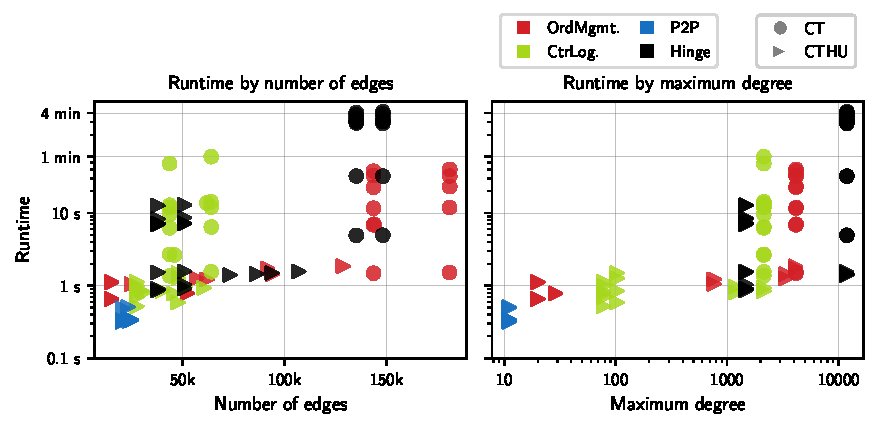
\includegraphics[width=\textwidth]{figures/20240910-175043-eva-scatter-edges-degree-runtime-61c1c0ba.pdf}
  \caption{Runtime of \allocrule{ClosestTargets} in relation to the number of edges in the object interaction graph (left) and the maximum degree (right). Different colors indicate the OCELs used for evaluation, different marker shapes the two graph versions.}
  \label{fig:eva-scatter-edges-degree-runtime}
\end{figure}

For assessing the runtime results, both the graphs with and without object type self-loops are considered again.
\autoref{fig:eva-scatter-edges-degree-runtime}
shows the runtime distribution in relation to number of edges and maximum degree in the object interaction graph.
Runtime of the \allocrule{ClosestTargets} allocation reaches a maximal value of 4m10s when using the full graph to allocate to \otype{HingePacks} in the \textit{Hinge} OCEL.
Overall, the 16 highest runtimes are measured when allocating to the HUs of the \textit{Hinge} OCEL using the full graph. The lowest 28 runtimes are those from the \textit{P2P} OCEL, bounded by \qty{0.5}{\second}.
Order management has the largest graphs with up to 180k edges in the full object interaction graph. This leads to runtimes up to one minute.
Edge counts in container logistics are centered around 50k, with similar runtimes.

Degrees are highest in the hinge OCEL (up to 11k).
Among these graphs is one HU interaction graph. The object type causing this outlier is addressed in \autoref{ssec:eva-results-hinge}.
Every graph containing resources has degrees exceeding 1000.

\begin{figure}[t]
  \centering
  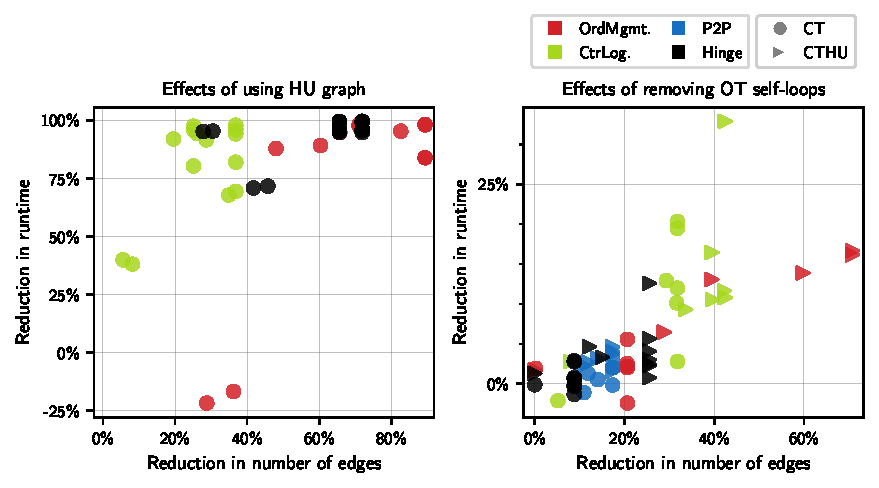
\includegraphics[width=\textwidth]{figures/20240910-180848-eva-scatter-both-effects-f7e4b0e7.pdf}
  \caption{Relative reduction in number of edges and runtime when using the HU graph over the full graph (left) and removing OT self-loops (right). OCELs are distinguished by colors, the P2P OCEL is omitted on the left as it only contains HUs.}
  \label{fig:eva-effects}
\end{figure}

\autoref{fig:eva-effects} shows the effects of choosing the HU interaction graph over the full graph, as well as removing object type self-loops.
The choice of the object interaction graph has significant influence on both the number of edges and allocation runtime.
In most runs, execution time drops by over \qty{65}{\percent}. The few outliers, including two in which runtime increases, all have an absolute runtime below \qty{2}{\second}. Therefore, this does not change the overall performance.
Many runs reach runtime savings close to \qty{100}{\percent}. On average, \qty{95.4}{\percent} of the runtime is saved (\qty{77.8}{\second} in absolute figures).

The P2P OCEL is not shown because all of its object types are HUs, making the HU interaction graph equal to the full object interaction graph. In the other datasets, the edge number of both graphs mostly differ by values between \qtyrange{20}{85}{\percent}.

Both values are also reduced when removing object type self-loops (on both graph types).
The differences are not as large as between the two graph types, but equally significant.
Runtime gets reduced by at most \qty{32.9}{\percent} (median \qty{2.8}{\percent}), edge numbers by at most \qty{70.8}{\percent} (median \qty{17.4}{\percent}).
If runtime increases, it does by at most \qty{2.4}{\percent}.

Edge number reduction is especially high in HU graphs,
as most object type self-loops are edges between HUs.
This is due to HUs of the same type appearing more often in the same event than do resources of the same type.
% A positive correlation of edge number reduction and runtime reduction is visible, with 

% ---------------------------------------------------------------------
\subsection{Order Management}
\label{ssec:eva-results-orderManagement}
% ---------------------------------------------------------------------

The \textit{order management} OCEL~\cite{orderManagement}
contains simulated data from a process that handles incoming orders from customers, from registering them to packing and shipping the packages and receiving payments.
A \otype{package} contains one or more \otype{items}, which are the tangible instances of \otype{products}.

\otype{Products}, as well as \otype{employees} and \otype{customers} are objects that recur within the process and do not enter nor leave the system. \autoref{tab:eva-input-orderManagementWithDistances-otypes} shows their high number of events and objects they interact with, making them resources.
\otype{Items} belong to a unique \otype{order} and are packed in a \otype{package}. All of theses three object types are case candidates in classical PM, with a maximum trace length of 16 events and 51 interacting objects, and are therefore labeled HUs.

\begin{table}[t]
  \centering
  \caption{Object types of \textit{order management} with their assigned class (HU or Resource), number of events per object (median [min-max]), percentage of events related to at least one object of the type, and number of related objects (degree in $\OGOmegaL$)}
  \label{tab:eva-input-orderManagementWithDistances-otypes}
  \small
  \begin{tabularx}{\textwidth}{XS[table-format=4]S[table-format=4.1]@{\,}lrS[table-format=4.1]@{\,}ll}
    \toprule
    \textbf{Object type} & \textbf{Count} & \multicolumn{2}{c}{\textbf{Events per object}} & \textbf{Ev. covered} & \multicolumn{2}{c}{\textbf{Degree}} & \textbf{Class} \\
    \midrule
    items & 7659 & 7 & [\numrange{7}{16}] & \qty{100}{\percent} & 25 & [\numrange{9}{51}] & HU \\
    orders & 2000 & 3 & [\numrange{3}{7}] & \qty{31}{\percent} & 8 & [\numrange{4}{27}] & HU \\
    packages & 1128 & 3 & [\numrange{3}{10}] & \qty{18}{\percent} & 15 & [\numrange{4}{37}] & HU \\
    products & 20 & 2716 & [\numrange{2439}{3009}] & \qty{100}{\percent} & 3857 & [\numrange{3530}{4174}] & Res. \\
    employees & 18 & 470.5 & [\numrange{267}{1906}] & \qty{78}{\percent} & 2230.5 & [\numrange{1262}{3399}] & Res. \\
    customers & 15 & 262 & [\numrange{206}{304}] & \qty{19}{\percent} & 646 & [\numrange{531}{792}] & Res. \\
    \bottomrule
  \end{tabularx}
\end{table}

For the \textit{order management} log, \autoref{tab:eva-results-alloc} shows that CTHU allocates the majority of events uniquely for each target object type setting. \otype{Customers} can uniquely be linked to each event.
In \otype{employees}, emission variation is highest, exceeding 0.6 for all non-trivial rules. Only one other object type across all OCELs yields higher variation.
This can be explained by different \otype{employee} roles (sales, shipment, and warehousing). Based on this attribute, an \otype{employee} takes part in a different number of events. A warehousing \otype{employee} takes part in at least 1766 events, the rest in at most 513 events.
When dividing allocated emissions by the number of events per object, variation is only 0.05.

In all target types, events are allocated over distances of at most 1. This is explained by the fact that at least one \otype{item} participates in every event, and each item is linked to some object of every other type.

The \textit{order management} OCEL has the largest full object interaction graphs. Also, edge reduction is highest with values up to \qty{89.4}{\percent} when using the HU graph over the full graph. The few resource objects are mostly linked to many HUs (e.g., each product has over 3500 items), while each HU is related to at most 20 objects per type in the HU graph.

\begin{figure}[t]
  \centering
  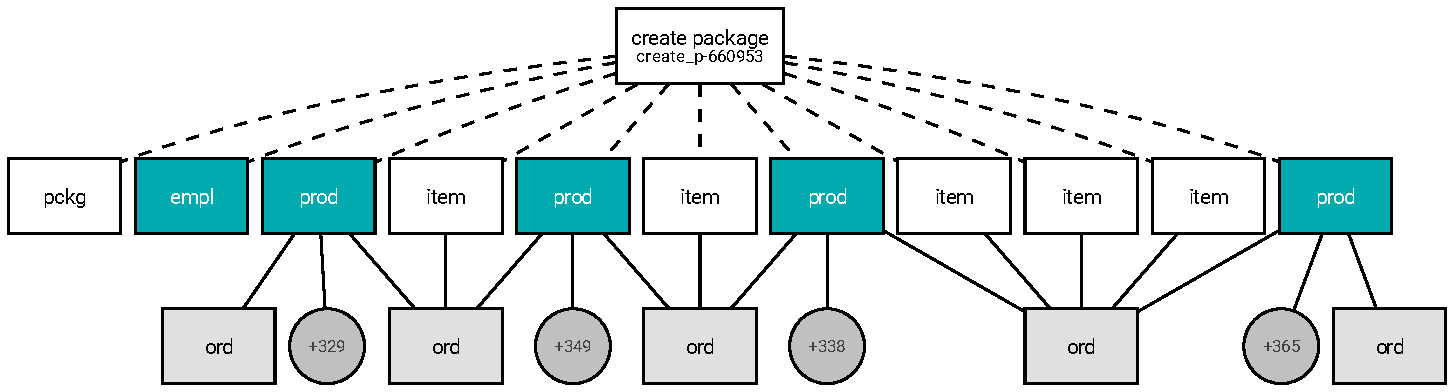
\includegraphics[width=\textwidth]{figures/20240910-210329-orderManagementWithDistances-og-subgraph-163fbff1.pdf}
  \caption{Paths in the full object interaction graph leading from objects participating in a \activity{create package} event to \otype{order} target objects (gray). Resources (turquoise) add many additional targets at distance 1.}
  \label{fig:orderManagementWithDistances-subgraph-createPackage}
\end{figure}

\autoref{fig:orderManagementWithDistances-subgraph-createPackage}
depicts how \allocrule{ClosestTargets} allocates emissions to \otype{order} target objects. Using the HU interaction graph, only three orders are found at distance 1 via \otype{item} objects.
Using the full object interaction graph, also resources like \otype{products} are considered.
Each product linked to the event adds more than 300 additional orders to the set of target objects at distance 1.

% ---------------------------------------------------------------------
\subsection{Container Logistics}
\label{ssec:eva-results-containerLogistics}
% ---------------------------------------------------------------------

The \textit{container logistics} OCEL~\cite{containerLogistics}
describes a process of a logistics company that ships goods using containers.
The goods are picked up at a production site and transferred to a terminal from where they are further transported by different company.

\otype{Customer orders} and \otype{transport documents} are artifacts documenting the process from registering an order, ordering \otype{containers}, transporting and storing \otype{handling units} in the terminal, to booking and finally loading \otype{vehicles}.
The process involves the use of \otype{forklifts} and \otype{trucks}. These are resources with long lifecycles and many related objects (see \autoref{tab:eva-input-containerLogistics-otypes}).
The aforementioned object types \otype{customer order}, \otype{transport document}, \otype{container} and \otype{handling unit}
\footnote{\otype{Handling unit} here refers to the name of an object type in the \textit{container logistics} OCEL~\cite{containerLogistics}. At the same time, this object type is labeled as handling unit (HU), the concept introduced in \autoref{sec:alloc-otcs}.}
are case-like types with shorter lifecycles and therefore considered HUs.

The \otype{vehicle} object type shows the ambiguity of the HU-resource distinction. \otype{Vehicles} are trains operated by a third-party company used for further transport. Judging by the quantities from \autoref{tab:eva-input-containerLogistics-otypes}, it significantly falls inbetween those object types labeled as HUs and resources, both regarding the object count and median number of events per object.
Labeling them as resources is an intuitive choice based on the fact that vehicles usually have a long lifetime and are rather \textit{used} by a process than being \textit{processed}.
However, the degrees of \otype{vehicles} in $\OGOmegaL$ are rather small and similar to those of other HUs. Also, a \otype{vehicle's} lifespan in the process is limited as it has a fixed departure and the number of \otype{containers} it can load is bounded.
Based on these arguments, \otype{vehicles} are labeled HUs.

\begin{table}[t]
  \centering
  \caption{Object types of \textit{container logistics} with their assigned class (HU or Resource), number of events per object (median [min-max]), percentage of events related to at least one object of the type, and number of related objects (degree in $\OGOmegaL$)}
  \label{tab:eva-input-containerLogistics-otypes}
  \small
  \begin{tabularx}{\textwidth}{XS[table-format=5]S[table-format=4.1]@{\,}lrS[table-format=4.1]@{\,}ll}
    \toprule
    \textbf{Object type} & \textbf{Count} & \multicolumn{2}{c}{\textbf{Events per object}} & \textbf{Ev. covered} & \multicolumn{2}{c}{\textbf{Degree}} & \textbf{Class} \\
    \midrule
    Handl. Unit & 10552 & 2 & [\numrange{1}{2}] & \qty{60}{\percent} & 2 & [\numrange{1}{2}] & HU \\
    Container & 1996 & 14 & [\numrange{1}{14}] & \qty{65}{\percent} & 34 & [\numrange{2}{65}] & HU \\
    Cust. Order & 600 & 2 & [\numrange{1}{2}] & \qty{3}{\percent} & 1 && HU \\
    Transp. Doc. & 594 & 4 & [\numrange{2}{8}] & \qty{5}{\percent} & 30 & [\numrange{1}{103}] & HU \\
    Vehicle & 127 & 21 & [\numrange{4}{53}] & \qty{8}{\percent} & 26 & [\numrange{5}{59}] & HU \\
    Truck & 6 & 2084.5 & [\numrange{2038}{2139}] & \qty{35}{\percent} & 2085.5 & [\numrange{2039}{2140}] & Res. \\
    Forklift & 3 & 2565 & [\numrange{2546}{2610}] & \qty{22}{\percent} & 1193 & [\numrange{1180}{1199}] & Res. \\
    \bottomrule
  \end{tabularx}
\end{table}

% ---------------------------------------------------------------------
\subsection{Procure-to-Pay (P2P)}
\label{ssec:eva-results-p2p}
% ---------------------------------------------------------------------

The Procure-to-Pay (P2P) OCEL~\cite{p2p} is the smallest of the four datasets (14671 events, 9054 objects). It is motivated by real-world procurement processes that use SAP software. It contains \otype{purchase requisitions} getting created and approved, \otype{quotations} being created and sent to a vendor, up to \otype{invoices} and \otype{payments} being processed.
All objects in the OCEL are considered HUs: All have short lifecycles (maximum 11 events per object, see \autoref{tab:eva-input-p2p-otypes}), and low degrees in the object interaction graph (maximum 11).

\begin{table}[t]
  \centering
  \caption{Object types of \textit{P2P}, all labeled as HU, together with the number of events per object (median [min-max]), percentage of events related to at least one object of the type, and number of related objects (degree in $\OGOmegaL$)}
  \label{tab:eva-input-p2p-otypes}
  \small
  \begin{tabularx}{\textwidth}{XS[table-format=4]S[table-format=4]@{\,}lrS[table-format=4]@{\,}ll}
    \toprule
    \textbf{Object type} & \textbf{Count} & \multicolumn{2}{c}{\textbf{Events per object}} & \textbf{Ev. covered} & \multicolumn{2}{c}{\textbf{Degree}} & \textbf{Class} \\
    \midrule
    goods rcpt. & 1941 & 5 & [\numrange{4}{9}] & \qty{62}{\percent} & 6 & [\numrange{3}{9}] & HU \\
    material & 1807 & 2 && \qty{10}{\percent} & 5 & [\numrange{4}{7}] & HU \\
    purch. order & 1598 & 6 & [\numrange{4}{9}] & \qty{57}{\percent} & 8 & [\numrange{4}{11}] & HU \\
    invoice rcpt. & 927 & 5 & [\numrange{3}{11}] & \qty{34}{\percent} & 5 & [\numrange{3}{9}] & HU \\
    payment & 927 & 1 & [\numrange{1}{5}] & \qty{8}{\percent} & 5 & [\numrange{3}{9}] & HU \\
    purch. req. & 927 & 3 & [\numrange{1}{3}] & \qty{16}{\percent} & 3 & [\numrange{1}{5}] & HU \\
    quotation & 927 & 3 & [\numrange{3}{9}] & \qty{28}{\percent} & 4 & [\numrange{2}{9}] & HU \\
    \bottomrule
  \end{tabularx}
\end{table}

In addition to not containing resources, the P2P OCEL exhibits a very regular structure.
The numbers of four of the seven object types are equal (927), also being the number of components in the object interaction graph, with each component containing exactly one object of the types in question.
Components are small (at most 16 objects). This makes BFS fast, with the runtime bounded by \qty{0.5}{\second}.
Events are always allocated uniquely by \allocrule{ClosestTargets} to those target types unique to components.
For the other types, no uniform allocation is observed, except for \otype{material} (\qty{19}{\percent} of events). \otype{materials} are only present in \qty{21}{\percent} of the connected components, all other object types in \qty{100}{\percent}.

% ---------------------------------------------------------------------
\subsection{Hinge Manufacturing}
\label{ssec:eva-results-hinge}
% ---------------------------------------------------------------------

The \textit{Hinge}~\cite{hinge} OCEL is the largest dataset, with 38528 events and 23771 objects.
It simulates a hinge manufacturing process, where \otype{hinges} are produced from the raw material, a \otype{steel coil}, that is cut into \otype{steel sheets} and then further processed into \otype{female} and \otype{male parts}. After assembling, the hinges are packed into \otype{hinge packs}, which is the process output. All aforementioned object types have short traces (\autoref{tab:eva-input-hinge-otypes}), making them HUs.
The \otype{steel coil} type is not a common HU example judging by quantities. \otype{Steel coils} are split into over 1400 \otype{steel sheets} each, leading to a high number of events and a high degree.
Still, the relation between these two types is considered meaningful as it represents input and output of a production step, and each \otype{steel sheet} is only related to exactly one \otype{steel coil}. Therefore, \otype{steel coil} is labeled an HU, too.
% \footnote{Intuitively, a material-like object type is a handling unit. Material and resource are synonyms in the context of production; here, resource refers to the opposite concept of objects supporting the process.}
% because of its high number of events and interacting objects (each of the only four \otype{steel coils} is split into over 1400 \otype{steel sheets}.)
Other object types like \otype{Machine}, \otype{WorkStation} and \otype{Worker} are prototypical examples of resources, with many events and high object interaction graph degrees.
As there is only one object of the types \otype{Facility} and \otype{Worker}, these objects are not tested as target objects in the experiment -- allocation would be trivial.

% \newpage

\begin{table}[t]
  \centering
  \caption{Object types of \textit{Hinge} with their assigned class (HU or Resource), number of events per object (median [min-max]), percentage of events related to at least one object of the type, and number of related objects (degree in $\OGOmegaL$)}
  \label{tab:eva-input-hinge-otypes}
  \small
  \begin{tabularx}{\textwidth}{XS[table-format=4]S[table-format=5]@{\,}lrS[table-format=5]@{\,}ll}
    \toprule
    \textbf{Object type} & \textbf{Count} & \multicolumn{2}{c}{\textbf{Events per object}} & \textbf{Ev. covered} & \multicolumn{2}{c}{\textbf{Degree}} & \textbf{Class} \\
    \midrule
    FormedPart & 5911 & 3 & [\numrange{2}{3}] & \qty{46}{\percent} & 7 & [\numrange{4}{7}] & HU \\
    SteelSheet & 5911 & 3& & \qty{46}{\percent} & 6& & HU \\
    FemalePart & 2915 & 3 & [\numrange{2}{3}] & \qty{23}{\percent} & 9 & [\numrange{4}{9}] & HU \\
    MalePart & 2914 & 3 & [\numrange{2}{3}] & \qty{23}{\percent} & 9 & [\numrange{4}{9}] & HU \\
    Hinge & 2907 & 2 & [\numrange{1}{2}] & \qty{8}{\percent} & 16 & [\numrange{5}{16}] & HU \\
    SteelPin & 2907 & 1& & \qty{8}{\percent} & 5& & HU \\
    HingePack & 290 & 1& & \qty{1}{\percent} & 12& & HU \\
    SteelCoil & 4 & 1478 & [\numrange{1477}{1478}] & \qty{15}{\percent} & 1480 & [\numrange{1479}{1480}] & HU \\
    Machine & 7 & 5911 & [\numrange{290}{5911}] & \qty{85}{\percent} & 5916 & [\numrange{3191}{11823}] & Res. \\
    Workstation & 3 & 11658 & [\numrange{3197}{23644}] & \qty{100}{\percent} & 11831 & [\numrange{11661}{11921}] & Res. \\
    Facility & 1 & 29& & \qty{0}{\percent} & 4& & Res. \\
    Worker & 1 & 5858& & \qty{15}{\percent} & 5831& & Res. \\
    \bottomrule
  \end{tabularx}
\end{table}

\autoref{fig:eva-input-hinge-otg-hu}
shows a summarized version of the HU interaction graph of the hinge OCEL.
Objects are grouped by type, connecting two types if any object pair of those types has an edge in $\OGHUOmegaL$.
This graph exhibits the structure of interactions in the log, showing the production process: The input (a steel coil) gets transformed to steel sheets, then female and male parts, and finally hinges that are packed to hinge packs.
This also explains the high path distances shown in \autoref{tab:eva-results-alloc}:
The highest value (8) is reached in allocation to hinge packs, aligning with the fact that they represent one end of this process.
Combined with the fact that the hinge OCEL is the largest among the four tested,
the high distances also explain the high runtimes visible in \autoref{fig:eva-scatter-edges-degree-runtime}.

\begin{figure}[t]
  \begin{small}
    \begin{center}
      \begin{tikzpicture}[
        % event/.style={rectangle,draw,inner sep=0,minimum size=.6cm},
        % every node/.style={node distance=2cm and 2cm},
        objectType/.style={rectangle,draw,font=\scriptsize,align=center,minimum height=.8cm},
        hu/.style={objectType,fill=rwthorange!50},
      ]
        \node[hu] (SteelCoil) {Steel\\Coil};
        \node[hu, right=1cm of SteelCoil] (SteelSheet) {Steel\\Sheet};
        \node[hu, right=1cm of SteelSheet] (FormedPart) {Formed\\Part};
        \node[hu, right=1.5cm of FormedPart] (SteelPin) {Steel\\Pin};
        % \node[hu, yshift=1.25cm] (FemalePart) at ($(FormedPart.east)!.5!(SteelPin.west)$) {FemalePart};
        % \node[hu, yshift=-1.25cm] (MalePart) at ($(FormedPart.east)!.5!(SteelPin.west)$) {MalePart};
        \node[hu, above=.5cm of SteelPin] (FemalePart) {FemalePart};
        \node[hu, below=.5cm of SteelPin] (MalePart) {MalePart};
        \node[hu, right=1cm of SteelPin] (Hinge) {Hinge};
        \node[hu, right=1cm of Hinge] (HingePack) {Hinge\\Pack};
        \draw
          (SteelCoil) edge (SteelSheet)
          (SteelSheet) edge (FormedPart)
          (FormedPart) |- ($(FemalePart.south west)!.67!(FemalePart.north west)$)
          (FormedPart) |- ($(MalePart.south west)!.33!(MalePart.north west)$)
          ($(FemalePart.south west)!.33!(FemalePart.north west)$) -| ($(FormedPart.east)!.5!(SteelPin.west)$) |- ($(MalePart.south west)!.67!(MalePart.north west)$)
          (FemalePart) -| (Hinge)
          (MalePart) -| (Hinge)
          (SteelPin) edge (FemalePart)
          (SteelPin) edge (MalePart)
          (SteelPin) edge (Hinge)
          (Hinge) edge (HingePack);
      \end{tikzpicture}
    \end{center}
    \caption{HU interaction graph of the \textit{Hinge} OCEL, summarized by object types. Two object types are connected when any object pair of the respective types has an edge in $\OGHUOmegaL$. The visualization shows that objects of the types \otype{SteelCoil} and \otype{HingePack} have at least a distance of 5 in $\OGHUOmegaL$.}
    \label{fig:eva-input-hinge-otg-hu}
  \end{small}
\end{figure}
